\documentclass[letterpaper,12pt]{article}

\usepackage{amsmath,amsfonts,mathtools}
\usepackage{amsthm}
\usepackage{amssymb}
\usepackage{graphicx}
\usepackage{hyperref}
\usepackage{enumitem}
\usepackage{float}
\usepackage{tikz}

% For displaying code
\usepackage{listings}
\usepackage{color}

% For pseudo code
\usepackage{algorithm}
\usepackage[noend]{algpseudocode}

\definecolor{dkgreen}{rgb}{0,0.6,0}
\definecolor{gray}{rgb}{0.5,0.5,0.5}
\definecolor{mauve}{rgb}{0.58,0,0.82}
\definecolor{orangered}{rgb}{1,0.27,0}

% Settings for displaying code
\lstset{language=python}

% Display tildes nicely
\lstset{
    literate={~} {$\sim$}{1}
}

\newcommand*{\lstitem}[1]{
  \setbox0\hbox{\lstinline{#1}}
  \item[\usebox0]
}

% Personal definitions
\newcommand{\lra}{\ensuremath{\longrightarrow{}}}
\newcommand{\vect}[1]{\mathbf{#1}}
\newcommand{\matr}[1]{\mathbf{#1}}
\newcommand{\norm}[1]{\left\lVert#1\right\rVert}
\newcommand{\abs}[1]{\lvert#1\rvert}
\newcommand*{\vertbar}{\rule[-1ex]{0.5pt}{2.5ex}} % for complicated matrices
\newcommand*{\horzbar}{\rule[.5ex]{2.5ex}{0.5pt}}
\renewcommand{\qedsymbol}{\rule{0.7em}{0.7em}}
\newcommand{\tabitem}{~~\llap{\textbullet}~~}

\makeatletter
\def\idots{\mathinner{\mkern1mu\raise\p@
\vbox{\kern7\p@\hbox{.}}\mkern2mu
\raise4\p@\hbox{.}\mkern2mu\raise7\p@\hbox{.}\mkern1mu}}
\makeatother

\newcommand\undermat[2]{%
  \makebox[0pt][l]{$\smash{\underbrace{\phantom{%
    \begin{matrix}#2\end{matrix}}}_{\text{$#1$}}}$}#2}

\DeclareMathOperator{\tr}{tr}
\DeclareMathOperator{\rank}{rank}
\DeclareMathOperator{\diag}{diag}
\DeclareMathOperator{\dist}{dist}
\DeclareMathOperator{\simi}{sim}
\DeclareMathOperator{\merge}{merge}
\DeclareMathOperator{\dif}{dif}
\DeclareMathOperator{\ini}{in}

% Theorem commands
\newtheorem{lem}{Lemma}
\newtheorem{thm}{Theorem}
\newtheorem{defn}{Definition}

% Set spacing
\setenumerate{itemsep=1.5pt,parsep=1.5pt,topsep=0.5pt}
\setlist{itemsep=1.5pt,parsep=1.5pt,leftmargin=1pt}
\setitemize{itemsep=1.5pt,parsep=1.5pt,topsep=0.5pt}

% set 1" margins on 8.5" x 11" paper
% top left is measured from 1", 1"
\topmargin       0in
\oddsidemargin   0in
\evensidemargin  0in
\headheight      0in
\headsep         0in
\topskip         0in
\textheight      9in
\textwidth       6.5in

\begin{document}
\title{CS231A Notes}
\author{Sean Wu}
\date{\today}
\maketitle

\tableofcontents

\pagebreak

% set spacing
\setlength{\parindent}{0em}
\setlength{\parskip}{1em}

\section{Camera Models}
\subsection{Piece of Film (Camera Obscura) - da Vinci 1500s}
\begin{itemize}
 \item Camera obscura \lra means dark chamber
 \item Each point on the 3D object emits multiple rays of light outwards
 \item Add a barrier to block off most of the light rays
       \begin{itemize}
        \item Reduces blurring
        \item Establishes a one-to-one mapping between points on 3D object and the film
       \end{itemize}
       \begin{description}
        \item[aperture]: opening in barrier to allow some light rays to pass through and hit film
       \end{description}
       \begin{figure}[h!]
        \centering
        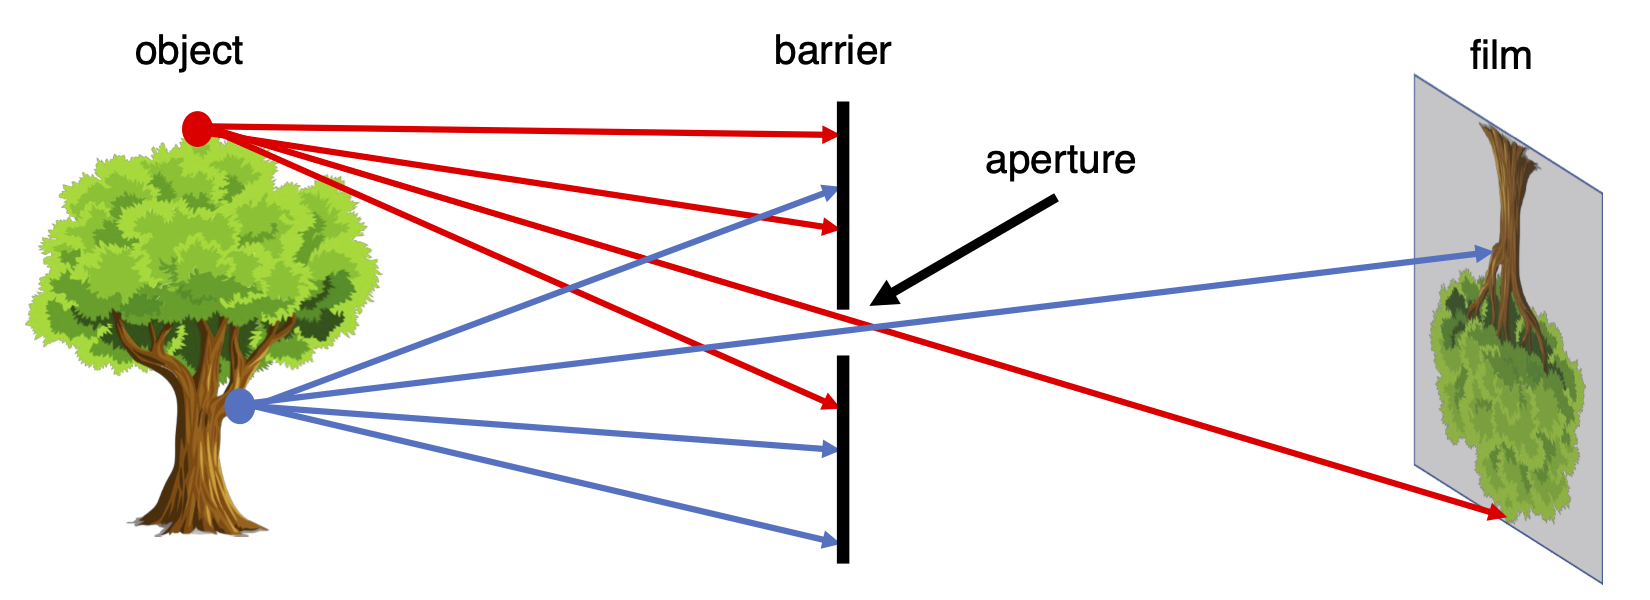
\includegraphics[width=0.8\textwidth]{images/camera_obscura.png}
        \caption{A simple working camera model: the pinhole camera model.}
       \end{figure}
\end{itemize}

\subsection{Pinhole Camera}
\begin{figure}[h!]
 \centering
 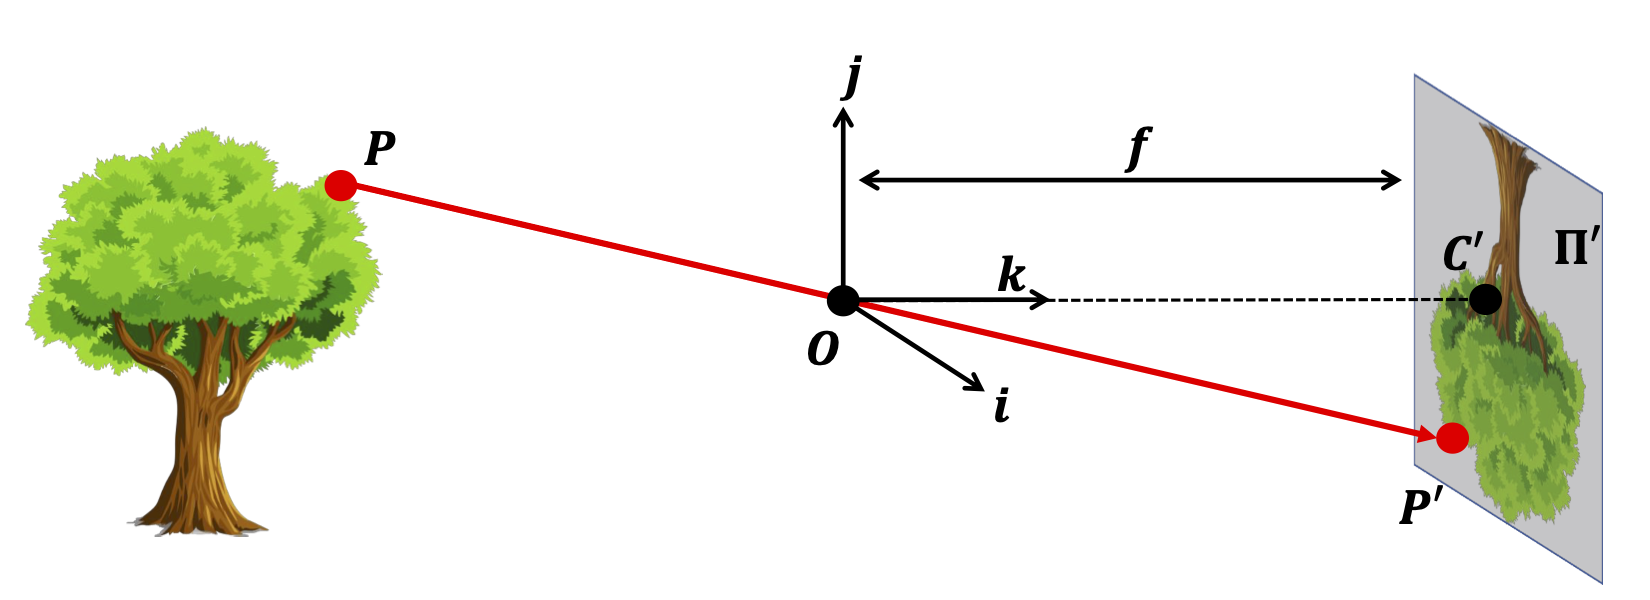
\includegraphics[width=0.8\textwidth]{images/pinhole_camera.png}
 \caption{A formal construction of the pinhole camera model.}
\end{figure}
\begin{description}
 \item[image or retinal plane]: the film inside the camera
 \item[$f$]: focal length
 \item[$O$]: aperture; pinhole centre of camera
 \item[virtual image or virtual retinal plane]: when image or retinal plane is placed in between the camera centre $O$ and the 3D object at a distance $f$ from $O$
 \item[optical axis]: the line defined by $C'$ and $O$
 \item[convention]: indicate projected or complementary points using the prime superscript (ex. $P'$ indicates point on image plane)
\end{description}
\begin{itemize}
 \item \textbf{Key Assumption:} the aperture in the pinhole model is a single point
       \begin{itemize}
        \item In most real world scenarios, we cannot assume that the aperture is infinitely small
        \item As aperture size increases \lra number of light rays passing through the barrier increases
        \item With more light rays passing through, each point on the film can be affected by light rays from multiple points in 3D space, blurring the image
        \item Smaller aperture \lra crisper but darker images
       \end{itemize}
 \item Note: projection of the object in the image plane and the image of the object in the virtual image plane are identical up to a scale (similarity) transformation
 \item Let $P = \begin{bmatrix}
         x & y & z
        \end{bmatrix}^T$ be a point on some 3D object visible to the pinhole camera
 \item $P$ gets mapped or \textbf{projected} onto the image plane $\Pi'$, resulting in point $P' = \begin{bmatrix}
         x' & y'
        \end{bmatrix}^T$
 \item Similarly, the pinhole itself can be projected onto th image plane, giving a new point $C'$
 \item Define a coordinate system $\begin{bmatrix}
         i & j & k
        \end{bmatrix}$ centered at the pinhole $O$ such that the axis $k$ is perpendicular to the image plane and points toward it
 \item Since the point $P'$ is obtained by the projection of the 3D point $P$,  on the image plane $\Pi'$, we can understand the way the 3D world is captured on the 2D image by finding the relationship between 3D point $P$ and image plane point $P'$
 \item Note: the triangle $P'C'O$ is similar to the triangle formed by $P$, $O$ and $(0,0,z)$
\end{itemize}


\begin{align}
 P = \underbrace{\begin{bmatrix}
   x \\
   y \\
   z
  \end{bmatrix}}_\text{3D}
 \lra
 P' = \underbrace{\begin{bmatrix}
   x' \\
   y'
  \end{bmatrix}}_\text{2D}
 =\begin{bmatrix}
  f \frac{x}{z} \\
  f \frac{y}{z}
 \end{bmatrix}\tag{$\mathbb{R}^3 \xrightarrow{E} \mathbb{R}^2$}
\end{align}
\begin{itemize}
 \item If aperture is too small, less light passes through
       \begin{itemize}
        \item Soln: use a lens
       \end{itemize}
\end{itemize}

\subsection{Lenses}
\begin{description}
 \item[lens]: focuses light onto the film; addresses crispness vs brightness tradeoff for smaller apertures
\end{description}
\begin{itemize}
 \item If pinhole is replaced with the right lens (position and size), it satisfies:
       \begin{itemize}
        \item \textbf{Property of Correct Lens:} all light rays emitted by a point $P$ are refracted by the lens such that they converge to a single point $P'$ in the image plane
        \item Note: this only occurs for a specific point $P$ that is in focus
        \item Another point $Q$ that is closer/further from the image plane than $P$ will be blurred or out of focus
       \end{itemize}
       \begin{figure}[h!]
        \centering
        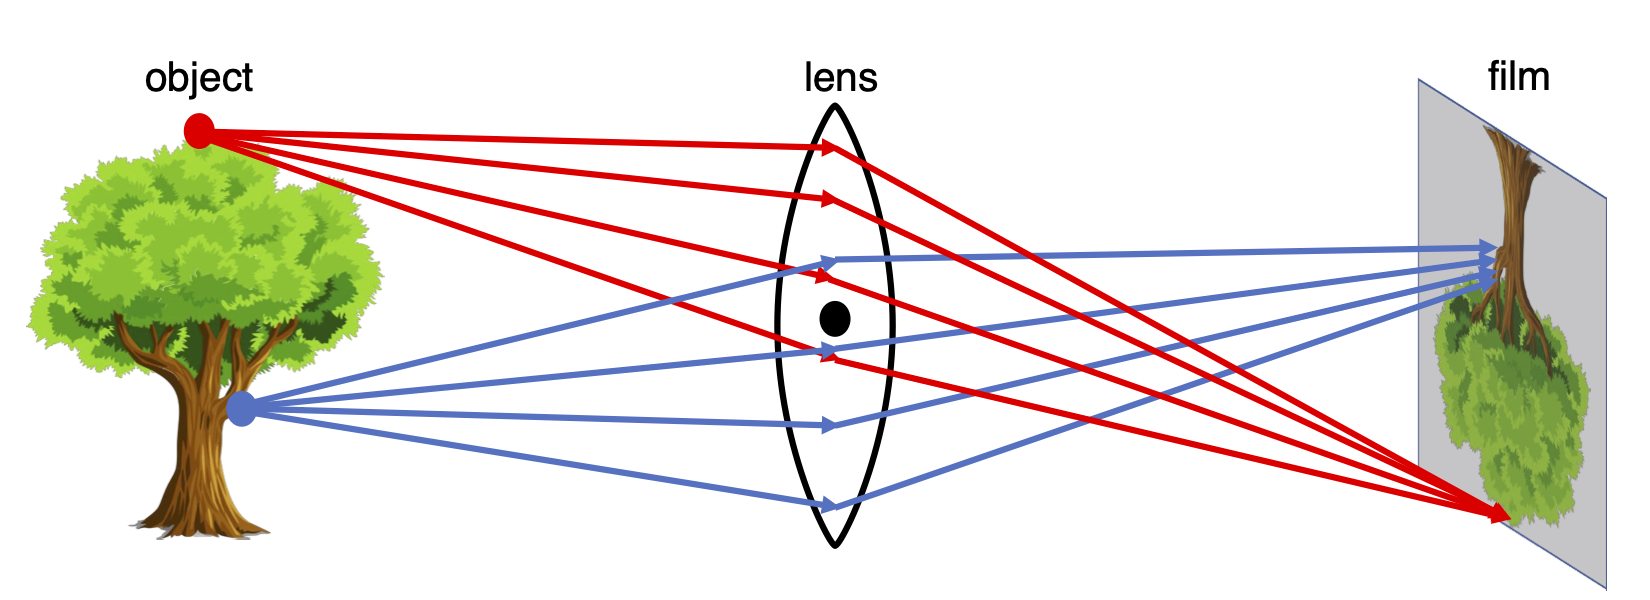
\includegraphics[width=0.8\textwidth]{images/lens.png}
        \caption{A setup of a simple lens model. Notice how the rays of the top point on the tree converge nicely on the film. However, a point at a different distance away from the lens results in rays not converging perfectly on the film (blurred).}
       \end{figure}
 \item Lenses have a special distance at which objects are ``in focus''
 \item Related to concept of depth of field
 \item All rays parallel to the optical (or principal) axis converge to one point (the \textbf{focal point}) on a plane located at the \textbf{focal length} $f$ from the centre of the lens
       \begin{itemize}
        \item Caused by light refraction in lens
       \end{itemize}
 \item Rays passing through the centre are not diverted
       \begin{figure}[h!]
        \centering
        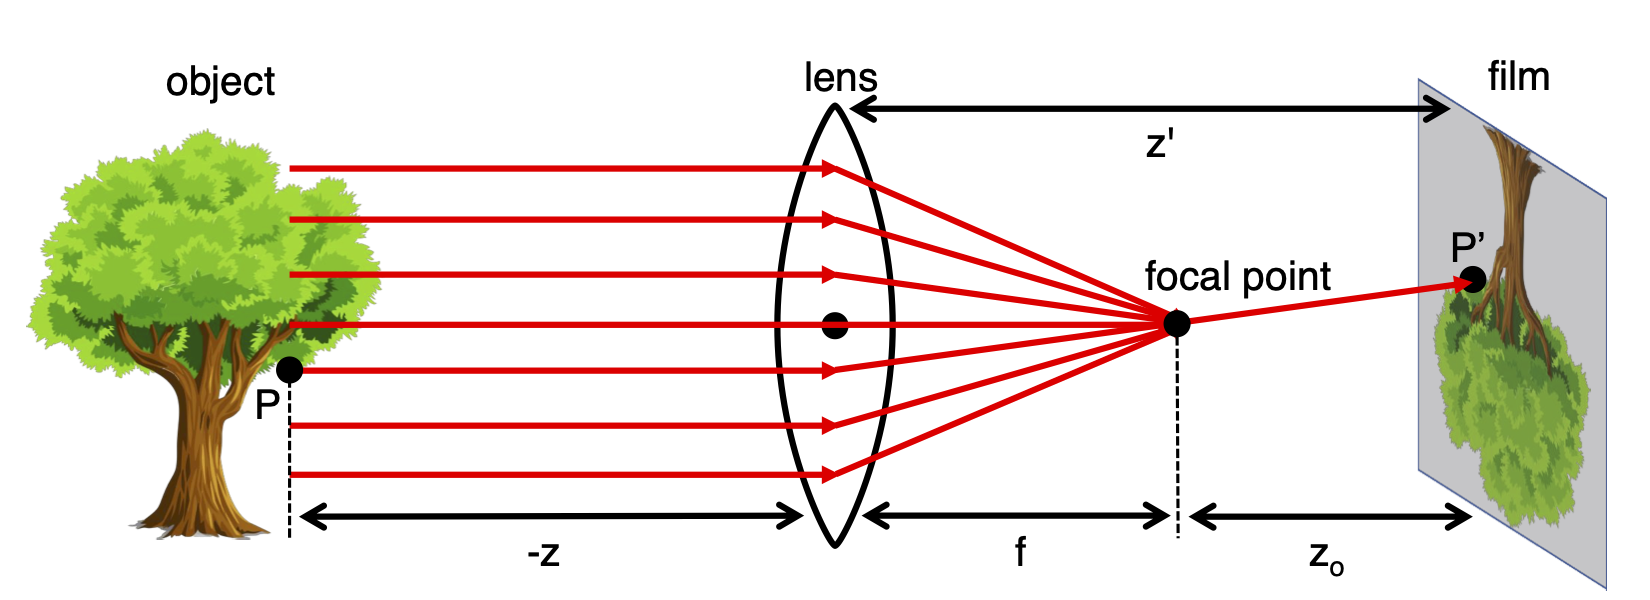
\includegraphics[width=0.8\textwidth]{images/parallel_light_ray.png}
        \caption{Lenses focus light rays parallel to the optical axis into the focal point. Furthermore, this setup illustrates the paraxial refraction model, which helps us find the relationship between points in the image plane and the 3D world in cameras with lenses.}
       \end{figure}
\end{itemize}

\subsubsection{Paraxial Refraction Model - Thin Lens Assumption}
\begin{itemize}
 \item With the lens, we can relate a point $P$ in 3D space with its corresponding image plane point $P'$ using Snell's law (w/ small angle approximation $sin\theta \approx \theta$ as $\theta \to 0$)
       \begin{align}
        \begin{cases}
         x' = z' \frac{x}{z} \quad\quad z' = f + z_0 \\
         y' = z' \frac{y}{z} \quad\quad f = \frac{R}{2(n-1)}
        \end{cases}
       \end{align}
\end{itemize}

\subsubsection{Issues with Lenses}
\begin{itemize}
 \item Because paraxial refraction model approximates using the thin lens assumption, many aberrations can occur
\end{itemize}

\subsubsection{Radial Distortion}
\begin{itemize}
 \begin{description}
  \item[radial distortion]: image magnification decreases/increases as a function of the distance to optical axis
  \item[pincushion distortion]: magnification increases further from the optical axis
  \item[barrel distortion]: magnification decreases further from the optical axis; usually occurs with fish-eye lenses
 \end{description}
 \item Deviations are most noticeable for rays that pass through the edge of the lens
       \begin{figure}[h!]
        \centering
        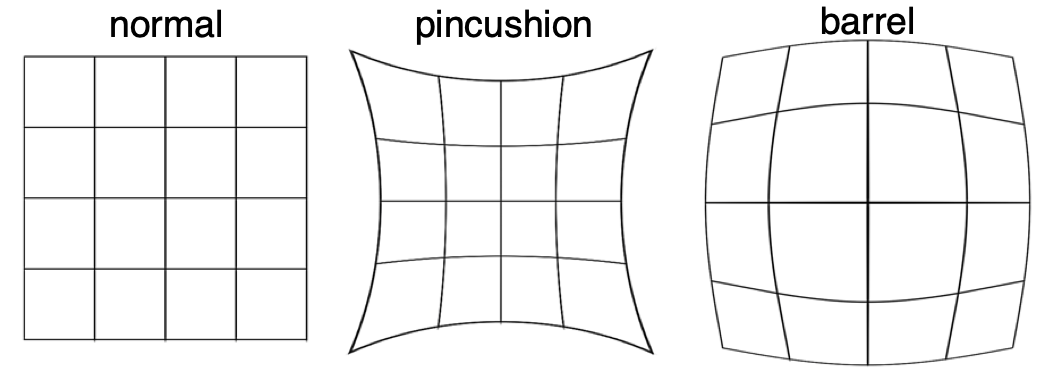
\includegraphics[width=0.8\textwidth]{images/radial_distortion.png}
        \caption{Demonstrating how pincushion and barrel distortions affect images.}
       \end{figure}
\end{itemize}

\subsection{Going to Digital Image Space}
\begin{itemize}
 \item Results derived using the pinhole model, but they hold as well for the paraxial refraction model
 \item A point $P$ in 3D space can be mapped (or projected) into a 2D point $P'$ in the image plane $\Pi'$ using a projective transformation
       \begin{description}
        \item[projective transformation]: a $\mathbb{R}^3 \to \mathbb{R}^2$ mapping of points in 3D space to 2D points in the image plane
       \end{description}
 \item Projective transformations do not directly correspond to what we see in actual digital images
       \begin{enumerate}
        \item Points in digital are, in general, in a different reference system than those in the image plane
        \item Digital images are divided into discrete pixels, whereas points in the image plane are continuous
        \item Physical sensors can introduce non-linearity (ex. distortion) to the mapping
       \end{enumerate}
 \item Thus have to introduce additional transformations to be able to map any point from the 3D world to pixel coordinates
\end{itemize}

\subsection{Coordinate systems}
\begin{itemize}
 \item Image coordinates have their origin $C'$ at the image centre where the $k$ axis intersects the image plane
 \item However, digital images typically have their origin at the lower-left corner of the image
 \item Thus, 2D points in the image plane and 2D points in the image are offset by a translation vector $\begin{bmatrix}
         c_x & c_y
        \end{bmatrix}^T$
       \begin{align}
        (x,y,z) \lra \bigg(f\frac{x}{z} + c_x, f\frac{y}{z} + c_y\bigg)
       \end{align}
 \item Points in digital images are expressed in pixels, while points in image plane are represented in physical measurements (ex. metres)
 \item Convert from metric to pixels with new parameters $k$ and $\ell$
       \begin{align}
        (x,y,z) \lra \bigg(\underbrace{fk}_\alpha \frac{x}{z} + c_x, \underbrace{f\ell}_\beta \frac{y}{z} + c_y\bigg)
        \label{eq:projective_transformation}
       \end{align}
 \item $[k]=[\ell]=\frac{\text{pixel}}{m}$ measure pixels
 \item Note: $k$ and $\ell$ may be different because the aspect ratio of the unit element is not guaranteed to be one
 \item If $k=\ell$, we say that the camera has \textbf{square pixels} (aspect ratio of 1)
 \item $[f]=m$ and $[\alpha]=[\beta]=\text{pixels}$
\end{itemize}

\subsubsection{Is this Projective Transformation Linear?}
\begin{align}
 P=(x,y,z) \lra P'=(\alpha \frac{x}{z} + c_x, \beta \frac{y}{z} + c_y)
\end{align}
\begin{enumerate}
\item Is the projection $P \to P'$ a linear transformation?
\begin{itemize}
\item No because the division of the input parameter $z$ is not linear
\item Can we express it with a matrix?
\begin{itemize}
 \item Yes, use homogenous coordinates
\end{itemize}
\end{enumerate}

\subsection{Homogenous Coordinates}
\begin{itemize}
 \item Consider transformations between Euclidean $\mathbb{E}$ and Homogenous $\mathbb{H}$ coordinates
       \begin{enumerate}
        \item $\mathbb{E} \lra \mathbb{H}$
              \begin{align}
               \underbrace{(x,y) \lra \begin{bmatrix}
                 x \\
                 y \\
                 1
                \end{bmatrix}}_\text{homogenous image coordinates}
               \quad\quad\quad
               \underbrace{(x,y,z) \lra \begin{bmatrix}
                 x \\
                 y \\
                 z \\
                 1
                \end{bmatrix}}_\text{homogenous scene coordinates}
              \end{align}
        \item $\mathbb{H} \lra \mathbb{E}$
              \begin{align}
               \begin{bmatrix}
                x \\
                y \\
                w
               \end{bmatrix}
               \lra \bigg(\frac{x}{w}, \frac{y}{w}\bigg)
               \quad\quad\quad
               \begin{bmatrix}
                x \\
                y \\
                z \\
                w
               \end{bmatrix}
               \lra \bigg(\frac{x}{w}, \frac{y}{w}, \frac{z}{w}\bigg)
              \end{align}
       \end{enumerate}
 \item Note: equality between a vector and its homogenous coordinates only occurs when the final coordinate is 1
\end{itemize}

\subsubsection{Projective Transformation in Homogenous Coordinate System}
\begin{itemize}
 \item Represent the projective transformation from eqn \ref{eq:projective_transformation} in Homogenous Coordinates as follows
\end{itemize}
\begin{align}
 P'_h = \underbrace{\begin{bmatrix}
   \alpha x + c_x z \\
   \beta y + c_y z  \\
   z
  \end{bmatrix}}_\text{Homogenous Image Coords}
 = \underbrace{\begin{bmatrix}
   \alpha & 0     & c_x & 0 \\
   0      & \beta & c_y & 0 \\
   0      & 0     & 1   & 0
  \end{bmatrix}}_\matr{M}
 \underbrace{\begin{bmatrix}
   x \\
   y \\
   z \\
   1
  \end{bmatrix}}_\text{Homogenous Scene Coords}
 = \begin{bmatrix}
  \alpha & 0     & c_x & 0 \\
  0      & \beta & c_y & 0 \\
  0      & 0     & 1   & 0
 \end{bmatrix}
 P_h
 \label{eq:homogenous_projective_transformation}
\end{align}
\begin{itemize}
 \item Can then convert Homogenous image coordinates to Euclidean image coordinates by dividing by $z$
       \begin{align}
        \underbrace{P'_h}_{Homogenous} \lra \underbrace{P' = (\alpha x + c_x z, \beta y + c_y z)}_\text{Euclidean}
       \end{align}
\end{itemize}

\subsection{Camera Matrix}
\begin{itemize}
 \item Note: from now on, assume we are using homogenous coordinates (unless stated otherwise)
 \item Drop the $h$ index, so any point $P$ or $P'$ can be assumed to be in homogenous coordinates
 \item From eqn \ref{eq:homogenous_projective_transformation}, can represent the relationship between a point in 3D space and its image coordinates by a vector relationship
       \begin{align}
        P' & = \begin{bmatrix}
         x' \\
         y' \\
         z
        \end{bmatrix}
        = \begin{bmatrix}
         \alpha & 0     & c_x & 0 \\
         0      & \beta & c_y & 0 \\
         0      & 0     & 1   & 0
        \end{bmatrix}
        \begin{bmatrix}
         x \\
         y \\
         z \\
         1
        \end{bmatrix}
        = \begin{bmatrix}
         \alpha & 0     & c_x & 0 \\
         0      & \beta & c_y & 0 \\
         0      & 0     & 1   & 0
        \end{bmatrix} P
        = \matr{M} P
       \end{align}
 \item Can then decompose this transformation into
       \begin{align}
        P' = \matr{M} P
        =\begin{bmatrix}
         \alpha                & 0     & c_x & 0 \\
         0                     & \beta & c_y & 0 \\
         \undermat{\matr{K}}{0 & 0     & 1}  & 0
        \end{bmatrix}
        P
        = \begin{bmatrix}
         \alpha & 0     & c_x \\
         0      & \beta & c_y \\
         0      & 0     & 1
        \end{bmatrix}
        \begin{bmatrix}
         \matr{I}_{3 \times 3} & \matr{0}
        \end{bmatrix} P
        = K \begin{bmatrix}
         \matr{I}_{3 \times 3} & \matr{0}
        \end{bmatrix} P
       \end{align}
 \item In summary,
       \begin{align}
        P & = \matr{M} P                     \\
          & = K \begin{bmatrix}
         \matr{I}_{3 \times 3} & \matr{0}
        \end{bmatrix} P
       \end{align}
       \begin{description}
        \item[$\matr{K}$] camera matrix; contains some of the critical parameters that are useful to characterize a camera model
       \end{description}
 \item The rows of the camera matrix can also be directly obtained from the projective transformation eqn expressing the image plane coordinates $x',y'$ in terms of the scene coordinates
       \begin{align}
        \matr{K} = \begin{bmatrix}
         x' \\
         y' \\
         z
        \end{bmatrix}
        = \begin{bmatrix}
         \alpha & 0     & c_x \\
         0      & \beta & c_y \\
         0      & 0     & 1
        \end{bmatrix}
       \end{align}
 \item Note: currently missing 2 parameters from our formulation: \textbf{skewness} and \textbf{distortion}
\end{itemize}

\subsection{Camera Skewness}
\begin{itemize}
 \item An image is called skewed when the camera coordinate system is skewed
       \begin{itemize}
        \item Here the angle between the two axes are slightly larger or smaller than 90 degrees
       \end{itemize}
 \item Most cameras have zero-skew, but some degree of skewness may occur because of sensor manufacturing errors
 \item New camera matrix accounting for skewness is
\end{itemize}
\begin{align}
 P' = \begin{bmatrix}
  \alpha & -\alpha\cot\theta        & c_x & 0 \\
  0      & \frac{\beta}{\sin\theta} & c_y & 0 \\
  0      & 0                        & 1   & 0
 \end{bmatrix}
 \begin{bmatrix}
  x \\
  y \\
  z \\
  1
 \end{bmatrix}
\end{align}
\begin{align}
 \matr{K} = \begin{bmatrix}
  x' \\
  y' \\
  z
 \end{bmatrix}
 = \begin{bmatrix}
  \alpha & -\alpha\cot\theta        & c_x \\
  0      & \frac{\beta}{\sin\theta} & c_y \\
  0      & 0                        & 1
 \end{bmatrix}
\end{align}
\begin{itemize}
 \item Ignoring distortion effects, the camera matrix $\matr{K}$ has 5 DOF: $\alpha$ and $\beta$ for focal length, $c_x$ and $c_y$ for image plane offset, and $\theta$ for skewness
\end{itemize}

\subsection{Canonical Projective Transformation}
\begin{itemize}
 \item $P' = \matr{M} P$
 \item i.e. $\mathbb{R}^4 \xrightarrow{H} \mathbb{R}^3$
\end{itemize}
\begin{align}
 P' = \begin{bmatrix}
  x \\
  y \\
  z
 \end{bmatrix}=\underbrace{\begin{bmatrix}
   1 & 0 & 0 & 0 \\
   0 & 1 & 0 & 0 \\
   0 & 0 & 1 & 0
  \end{bmatrix}}_\matr{M}
 \begin{bmatrix}
  x \\
  y \\
  z \\
  1
 \end{bmatrix}
\end{align}
\begin{align}
 P'_i = \begin{bmatrix}
  \frac{x}{z} \\
  \frac{y}{z}
 \end{bmatrix}
\end{align}

\subsection{World Reference System}
\begin{itemize}
 \item Mapping so far defined within Cartesian reference system
 \item Need to introduce an additional mapping from world reference system to camera reference system
       \begin{figure}[h!]
        \centering
        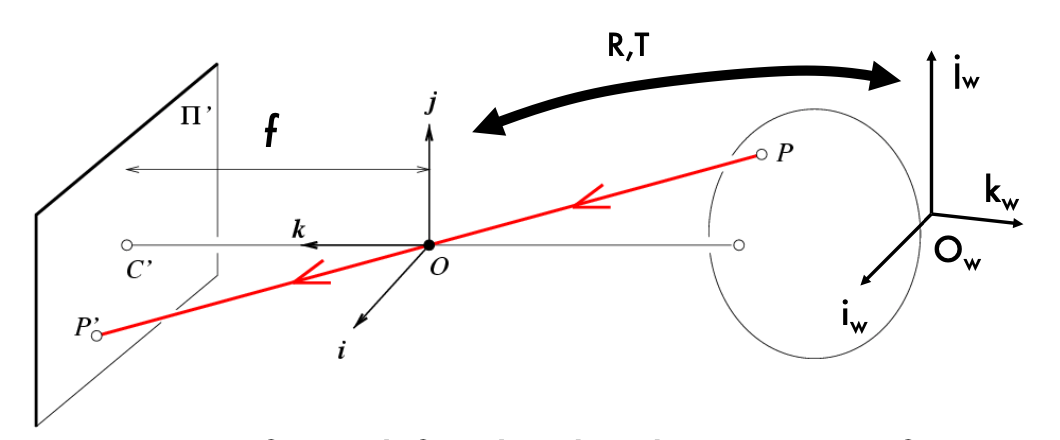
\includegraphics[width=0.8\textwidth]{images/world_reference_system.png}
        \caption{Mapping from world reference system $(i_w, j_w, k_w)$ to camera reference system $(i, j, k)$}
       \end{figure}
\end{itemize}

\subsection{2D Transformations}
\subsubsection{2D Translation}
\begin{itemize}
 \item $P = (x,y)$
 \item $\vect{t} = (t_x,t_y)$
 \item $P' = P + \vect{t} = (x + t_x, y + t_y)$
 \item Translation requires using homogenous coordinates
\end{itemize}
\begin{align}
 P' \lra \begin{bmatrix}
  x + t_x \\
  y + t_y \\
  1
 \end{bmatrix}
  & = \begin{bmatrix}
  1 & 0 & t_x \\
  0 & 1 & t_y \\
  0 & 0 & 1
 \end{bmatrix}
 \begin{bmatrix}
  x \\
  y \\
  1
 \end{bmatrix}      \\
  & = \begin{bmatrix}
  \matr{I} & \vect{t} \\
  0        & 1
 \end{bmatrix}
 \begin{bmatrix}
  x \\
  y \\
  1
 \end{bmatrix}
 = \matr{T} \begin{bmatrix}
  x \\
  y \\
  1
 \end{bmatrix}
\end{align}

\subsubsection{2D Scaling}
\begin{itemize}
 \item $P=(x,y) \lra P'=(s_x x, s_y y)$
 \item $P=(x,y) \lra (x,y,1)$
\end{itemize}
\begin{align}
 P' \lra \begin{bmatrix}
  s_x x \\
  s_y y \\
  1
 \end{bmatrix}
 = \underbrace{\begin{bmatrix}
   s_x & 0   & 0 \\
   0   & s_y & 0 \\
   0   & 0   & 1
  \end{bmatrix}}_\matr{S}
 \begin{bmatrix}
  x \\
  y \\
  1
 \end{bmatrix}
 = \begin{bmatrix}
  \matr{S}' & 0 \\
  0         & 1
 \end{bmatrix}
 \begin{bmatrix}
  x \\
  y \\
  1
 \end{bmatrix}
 = \matr{S}
 \begin{bmatrix}
  x \\
  y \\
  1
 \end{bmatrix}
\end{align}

\subsubsection{2D Rotation}
\begin{itemize}
 \item CCW rotation by angle $\theta$
 \item $x' = x\cos\theta -y\sin\theta$
 \item $y' = x\sin\theta \cos\theta$
\end{itemize}
\begin{align}
 \begin{bmatrix}
  x' \\
  y'
 \end{bmatrix}
 = \begin{bmatrix}
  \cos\theta & -\sin\theta \\
  \sin\theta & \cos\theta
 \end{bmatrix}
 \begin{bmatrix}
  x \\
  y
 \end{bmatrix}
\end{align}
\begin{itemize}
 \item $P' = \matr{R}P$
 \item 1 DOF
       \begin{align}
        P' = \lra \begin{bmatrix}
         \cos\theta & -\sin\theta & 0 \\
         \sin\theta & \cos\theta  & 0 \\
         0          & 0           & 1
        \end{bmatrix}
        \begin{bmatrix}
         x \\
         y \\
         1
        \end{bmatrix}
       \end{align}
\end{itemize}

\subsubsection{2D Scale + Rotation + Translation}
\begin{itemize}
 \item $P'= \matr{T}\matr{R}\matr{S}P$
\end{itemize}
\begin{align}
 P' & \lra \begin{bmatrix}
  1 & 0 & t_x \\
  0 & 1 & t_y \\
  0 & 0 & 1
 \end{bmatrix}
 \begin{bmatrix}
  \cos\theta & -\sin\theta & 0 \\
  \sin\theta & \cos\theta  & 0 \\
  0          & 0           & 1
 \end{bmatrix}
 \begin{bmatrix}
  S_x & 0   & 0 \\
  0   & S_y & 0 \\
  0   & 0   & 1
 \end{bmatrix}
 \begin{bmatrix}
  x \\
  y \\
  1
 \end{bmatrix}           \\
    & = \begin{bmatrix}
  \cos\theta & -\sin\theta & t_x \\
  \sin\theta & \cos\theta  & t_y \\
  0          & 0           & 1
 \end{bmatrix}
 \begin{bmatrix}
  S_x & 0   & 0 \\
  0   & S_y & 0 \\
  0   & 0   & 1
 \end{bmatrix}
 \begin{bmatrix}
  x \\
  y \\
  1
 \end{bmatrix}           \\
    & = \begin{bmatrix}
  \matr{R} & \matr{T} \\
  0        & 1
 \end{bmatrix}
 \begin{bmatrix}
  \matr{S} & 0 \\
  0        & 1
 \end{bmatrix}
 \begin{bmatrix}
  x \\
  y \\
  1
 \end{bmatrix}
 = \begin{bmatrix}
  \matr{R}\matr{S} & \matr{T} \\
  0                & 1
 \end{bmatrix}
 \begin{bmatrix}
  x \\
  y \\
  1
 \end{bmatrix}
\end{align}
\begin{itemize}
 \item Note: if $s_x = s_y$, this is a similarity transformation
\end{itemize}

\subsection{3D Transformations}
\subsubsection{3D Rotation of Points}
\begin{itemize}
 \begin{figure}[H]
  \centering
  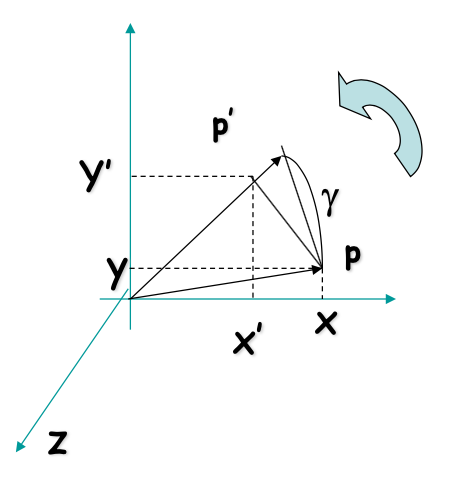
\includegraphics[width=0.5\textwidth]{images/3D_rotation.png}
  \caption{CCW rotation of $\gamma$ around the z-axis using $R_z(\gamma)$.}
 \end{figure}
 \item A rotation matrix in 3D has 3 DOF
 \item Rotation matrices for \textbf{CCW} rotation about the coordinate axes are:
\end{itemize}
\begin{align}
 R_x(\alpha) = \begin{bmatrix}
  1 & 0          & 0           \\
  0 & \cos\alpha & -\sin\alpha \\
  0 & \sin\alpha & \cos\alpha
 \end{bmatrix}
\end{align}

\begin{align}
 R_y(\beta) = \begin{bmatrix}
  \cos\beta  & 0 & \sin\beta \\
  0          & 1 & 0         \\
  -\sin\beta & 0 & \cos\beta
 \end{bmatrix}
\end{align}

\begin{align}
 R_z(\gamma) = \begin{bmatrix}
  \cos\gamma & -\sin\gamma & 0 \\
  \sin\gamma & \cos\gamma  & 0 \\
  0          & 0           & 1
 \end{bmatrix}
\end{align}
\begin{align}
 P' \lra \begin{bmatrix}
  \matr{R} & 0 \\
  0        & 1
 \end{bmatrix}_{4 \times 4}
 \begin{bmatrix}
  x \\
  y \\
  z \\
  1
 \end{bmatrix}
\end{align}

\subsubsection{3D Translation of Points}
\begin{align}
 \vect{T} = \begin{bmatrix}
  t_x \\
  t_y \\
  t_z
 \end{bmatrix}
\end{align}

\begin{align}
 P' \lra \begin{bmatrix}
  \matr{I} & \vect{T} \\
  0        & 1
 \end{bmatrix}_{4 \times 4}
 \begin{bmatrix}
  x \\
  y \\
  z \\
  1
 \end{bmatrix}
\end{align}
\begin{itemize}
 \item A translation vector in 3D has 3 DOF
\end{itemize}

\subsubsection{3D Translation and Rotation}
\begin{align}
 \vect{T} = \begin{bmatrix}
  t_x \\
  t_y \\
  t_z
 \end{bmatrix}
\end{align}

\begin{align}
 \matr{R} = R_x(\alpha) R_y(\beta) R_z(\gamma)
\end{align}

\begin{align}
 P' = \begin{bmatrix}
  \matr{R} & \vect{T} \\
  0        & 1
 \end{bmatrix}_{4 \times 4}
 \begin{bmatrix}
  x \\
  y \\
  z \\
  1
 \end{bmatrix}
\end{align}

\subsection{World Reference System}
\begin{itemize}
 \item In 4D homogenous coordinates
\end{itemize}
\begin{align}
 P = \begin{bmatrix}
  \matr{R} & \vect{T} \\
  0        & 1
 \end{bmatrix}_{4 \times 4}
 P_w
\end{align}

\begin{align}
 P_w = \begin{bmatrix}
  x_w \\
  y_w \\
  z_w \\
  1
 \end{bmatrix}
\end{align}

\begin{align}
 P' = \matr{K} \begin{bmatrix}
  \matr{I} & 0
 \end{bmatrix}
 P
 = \matr{K} \begin{bmatrix}
  \matr{I} & 0
 \end{bmatrix}
 \begin{bmatrix}
  \matr{R} & \vect{T} \\
  0        & 1
 \end{bmatrix}_{4 \times 4}
\end{align}

\begin{description}
 \item[$\matr{K}$] camera matrix (internal parameters)
 \item[$\matr{M}$] perspective projection matrix
 \item[$\matr{R}$, $\matr{T}$] rotation and translation matrix (external parameters)
\end{description}

\begin{align}
 P_w = \underbrace{\matr{K} \begin{bmatrix}
   \matr{R} & \vect{T}
  \end{bmatrix}}_\matr{M}
 P_w
\end{align}

\subsection{More about Projective Transformations}
\begin{align}
 P'_{3 \times 4} = \matr{M}_{3 \times 4} P_w = \matr{K}_{3 \times 3} \begin{bmatrix}
  \matr{R} & \vect{T}
 \end{bmatrix}_{3 \times 4}
\end{align}
\begin{itemize}
 \item Total DOF: $5 + 3 + 3 = 11$ 
\end{itemize}

\begin{align}
 \matr{M} = \begin{bmatrix}
  m_1 \\
  m_2 \\
  m_3
 \end{bmatrix}
\end{align}

\begin{align}
 P'_{3 \times 1} & = \matr{M} P_w                \\
                 & = \begin{bmatrix}
  m_1 P_w \\
  m_2 P_w \\
  m_3 P_w
 \end{bmatrix}
 \xrightarrow{E} (\frac{m_1 P_w}{m_3 P_w}, \frac{m_2 P_w}{m_3 P_w})
\end{align}

\subsubsection{Faugeras Theorem}
\begin{align}
 \matr{M} = \matr{K} \begin{bmatrix}
  \matr{R} & \vect{T}
 \end{bmatrix}
 = \begin{bmatrix}
  \matr{K}\matr{R} & \matr{K}\vect{T}
 \end{bmatrix}
 = \begin{bmatrix}
  \matr{A} & \vect{T}
 \end{bmatrix}
\end{align}
\begin{align}
 \matr{A} = \begin{bmatrix}
  a_1 \\
  a_2 \\
  a_3
 \end{bmatrix}
\end{align}
\begin{itemize}
 \item A necessary and sufficient condition for a matrix $\matr{M}$ to be a \textbf{perspective projection matrix} is that $\det(\matr{A}) \neq 0$
 \item A necessary and sufficient condition for a matrix $\matr{M}$ to be a \textbf{zero-skew perspective projection matrix} is that $\det(\matr{A}) \neq 0$ \textbf{AND}
       \begin{align}
        (a_1 \times a_3) \cdot (a_2 \times a_3) = 0 \tag{\text{Mutually Orthogonal}}
       \end{align}
 \item A necessary and sufficient condition for a matrix $\matr{M}$ to be a \textbf{perspective projection matrix} with \textbf{zero-skew} and \textbf{unit aspect ratio} is that $\det(\matr{A}) \neq 0$ \textbf{AND}
       \begin{align}
        \begin{cases}
         (a_1 \times a_3) \cdot (a_2 \times a_3) = 0 \\
         (a_1 \times a_3) \cdot (a_1 \times a_3) = (a_2 \times a_3) \cdot (a_2 \times a_3)
        \end{cases}
       \end{align}
\end{itemize}

\subsubsection{Properties of Projective Transformations}
\begin{itemize}
 \item Points project to points
 \item Lines project to lines
 \item Distant objects look further
 \item Angles are \textbf{NOT} preserved
 \item Parallel lines \textbf{meet}
\end{itemize}
\begin{description}
 \item[Vanishing point]: point at which parallel lines in the world intersect in an image
\end{description}



\end{document}
